\documentclass[10pt,a4paper]{article}

\usepackage{fontspec}
\usepackage[top=1cm]{geometry}
\usepackage[backend=bibtex]{biblatex}
\usepackage{hyperref}
\usepackage{graphicx}
\usepackage{subfig}
\defaultfontfeatures{Mapping=tex-text}
\setromanfont[Ligatures={Common},Numbers={Lining}]{Linux Libertine}
\author{Michal Staniaszek}
\title{Thesis Literature Review}

\bibliography{../report/report.bib}

\begin{document}
\maketitle
\section{Plane Extraction}
\section{Segmentation}
Popularised by Comaniciu~\cite{comaniciu2002mean} for use in image segmentation,
mean shift was first introduced by Fukunaga~\cite{fukunaga1975estimation} in
1975, and rediscovered by Cheng~\cite{cheng1995mean} in 1995. The technique finds
stationary points in a density estimate of the feature space, for example pixel
RGB values, and uses those points to define regions in the space by allocating
pixels to them. Pixels which follow the gradient of the density to the same
stationary point are part of the same segment. An example can be seen in
Figure~\ref{fig:meanshift}.
\begin{figure}
  \centering
  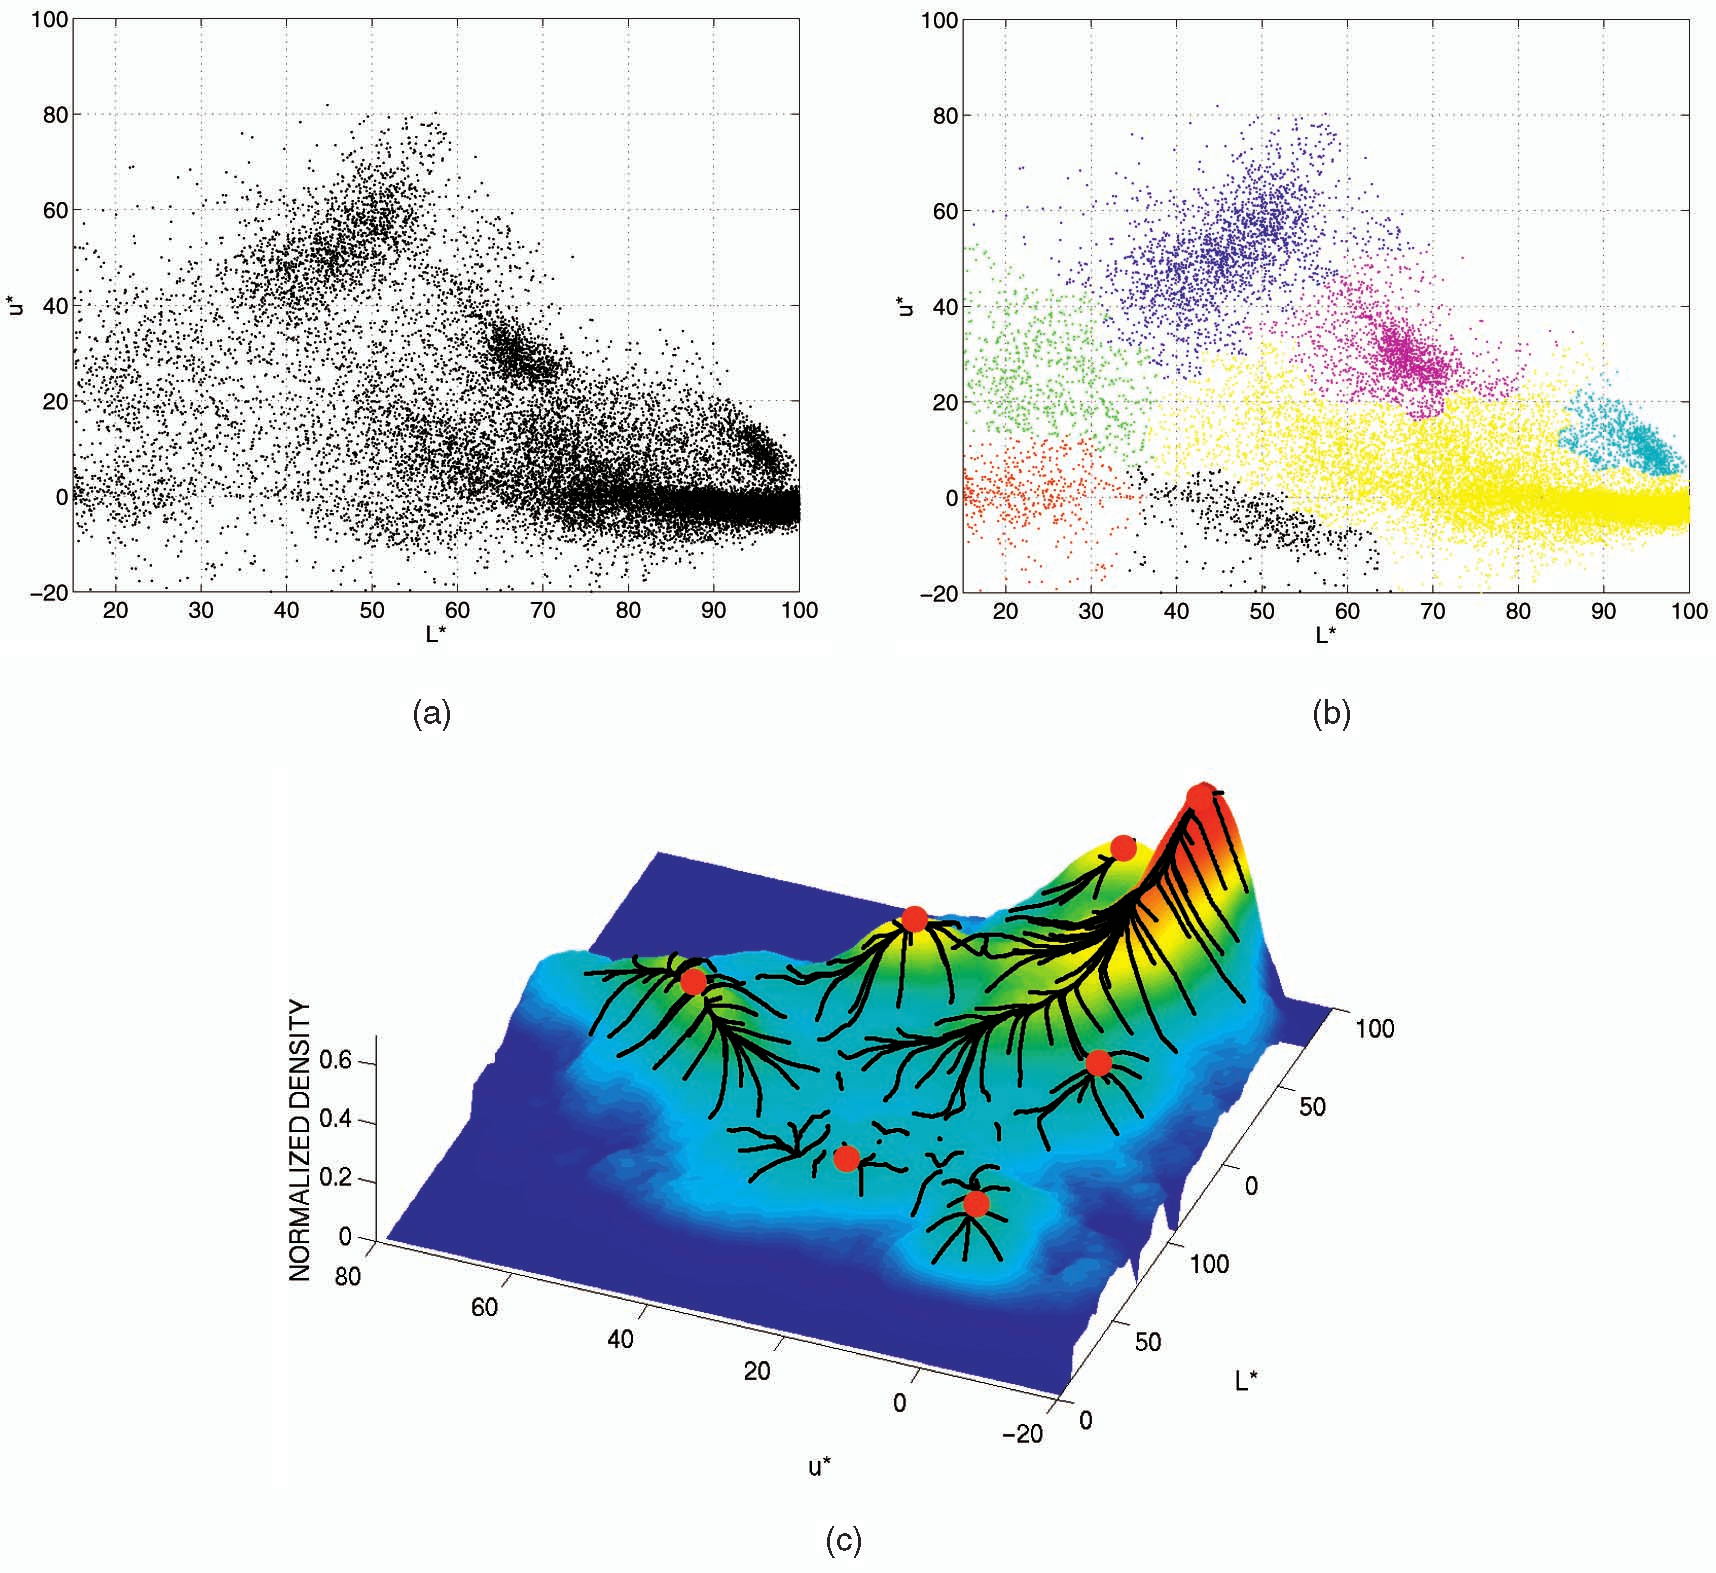
\includegraphics[width=\textwidth]{images/meanshift}
  \caption{Visualisation of mean shift \cite{comaniciu2002mean}. a) First two
    components of image pixels in LUV space. b) Decomposition found by running
    mean shift. c) Trajectories of mean shift over the density estimate.}
  \label{fig:meanshift}
\end{figure}
\section{Interest Points}
Mikolajczyk and Schmid~\cite{mikolajczyk2004scale} introduce an interest point
detector which is an improvement on SIFT \cite{lowe2004distinctive} and the
Laplacian of Gaussians \cite{lindeberg1998feature} in the sense that it is able
to deal with affine transformations. They do not, however, introduce a new type
of descriptor to go with the point selection.
\section{2D Descriptors}
Different considerations must be made for 2D images because of affine
transforms, rotation and so on

Van Gool \cite{van1996affine} gives a description of how to use moment
invariants to recognise planar patterns like labels and signs under affine
deformations. The moments describe things like the size of the shape and its centre
of mass, or statistics like the mean and variance of pixel intensities in the
shape. These moments can be combined in such a way that they are invariant to
deformations, which is useful to have in a descriptor.
\section{3D Descriptors}
The Ensemble of Shape Functions (ESF) descriptor introduced in
\cite{wohlkinger2011ensemble} combines the Shape Distribution approach
introduced by \cite{osada2002shape} along with some extensions proposed by
\cite{ip2002using}. Pairs or triples of points are sampled from segmented
partial clouds of objects, and histograms are created by extracting information
such as distance, angle, ratios, and whether points are inside or outside (or a
mix) of the model. See Figure~\ref{fig:wohlESF}.

Work in protein-protein docking also uses 3D descriptors to help with
simulations of an otherwise lengthy process. The Surface Histogram is introduced
by Gu et al. \cite{gu2012surface}, and uses the local geometry around two points
with specific normals on the surface of a protein. A coordinate system is
defined by the two points and the line between them, and a rectangular voxel
grid is defined around the points. The grid is then marked in locations where
the surface crosses the grid, and a 2D image is constructed by squashing the
data onto one of the axes. The descriptor is designed to immediately give a
potential pose for the docking.
 
\begin{figure}
  \centering
  \subfloat[]{
    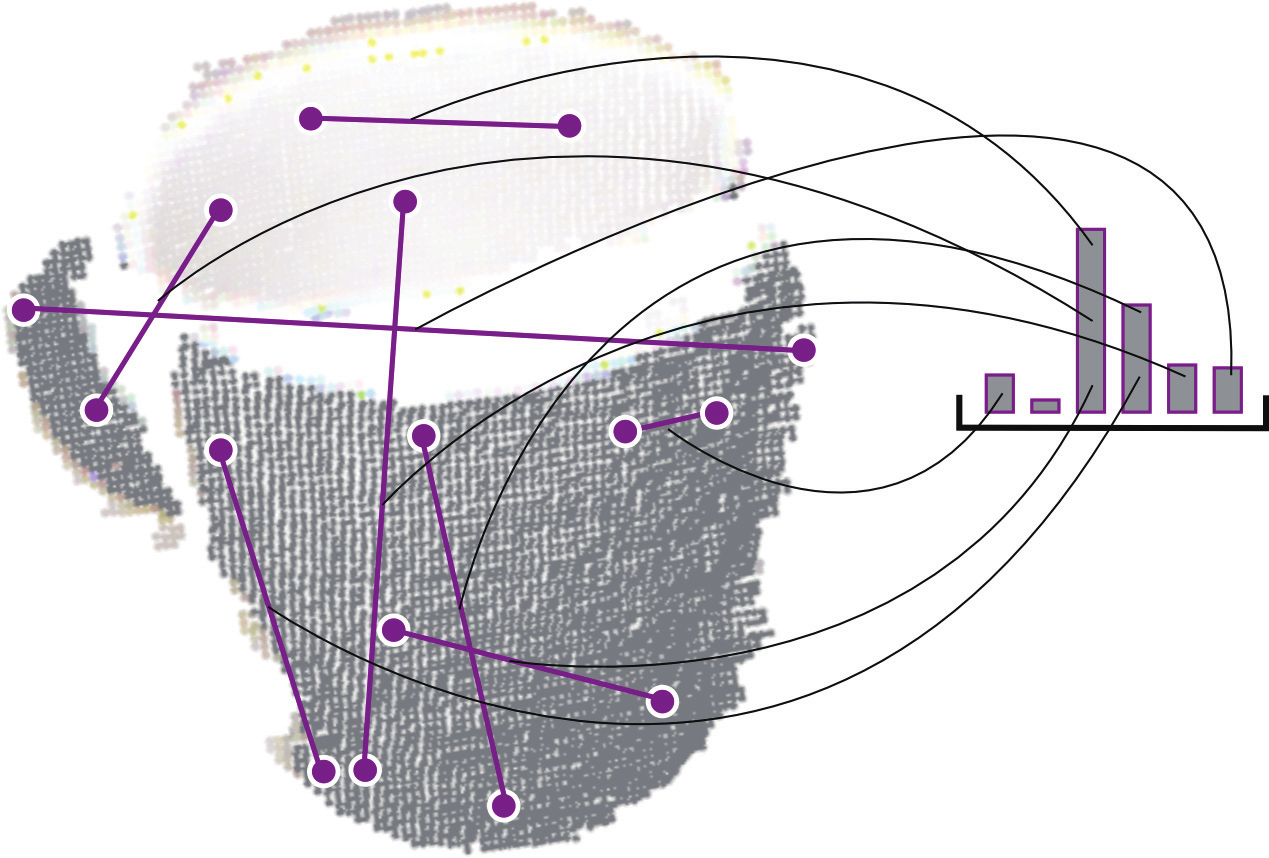
\includegraphics[width=0.23\textwidth]{images/wohl_d2}
  }
  \subfloat[]{
    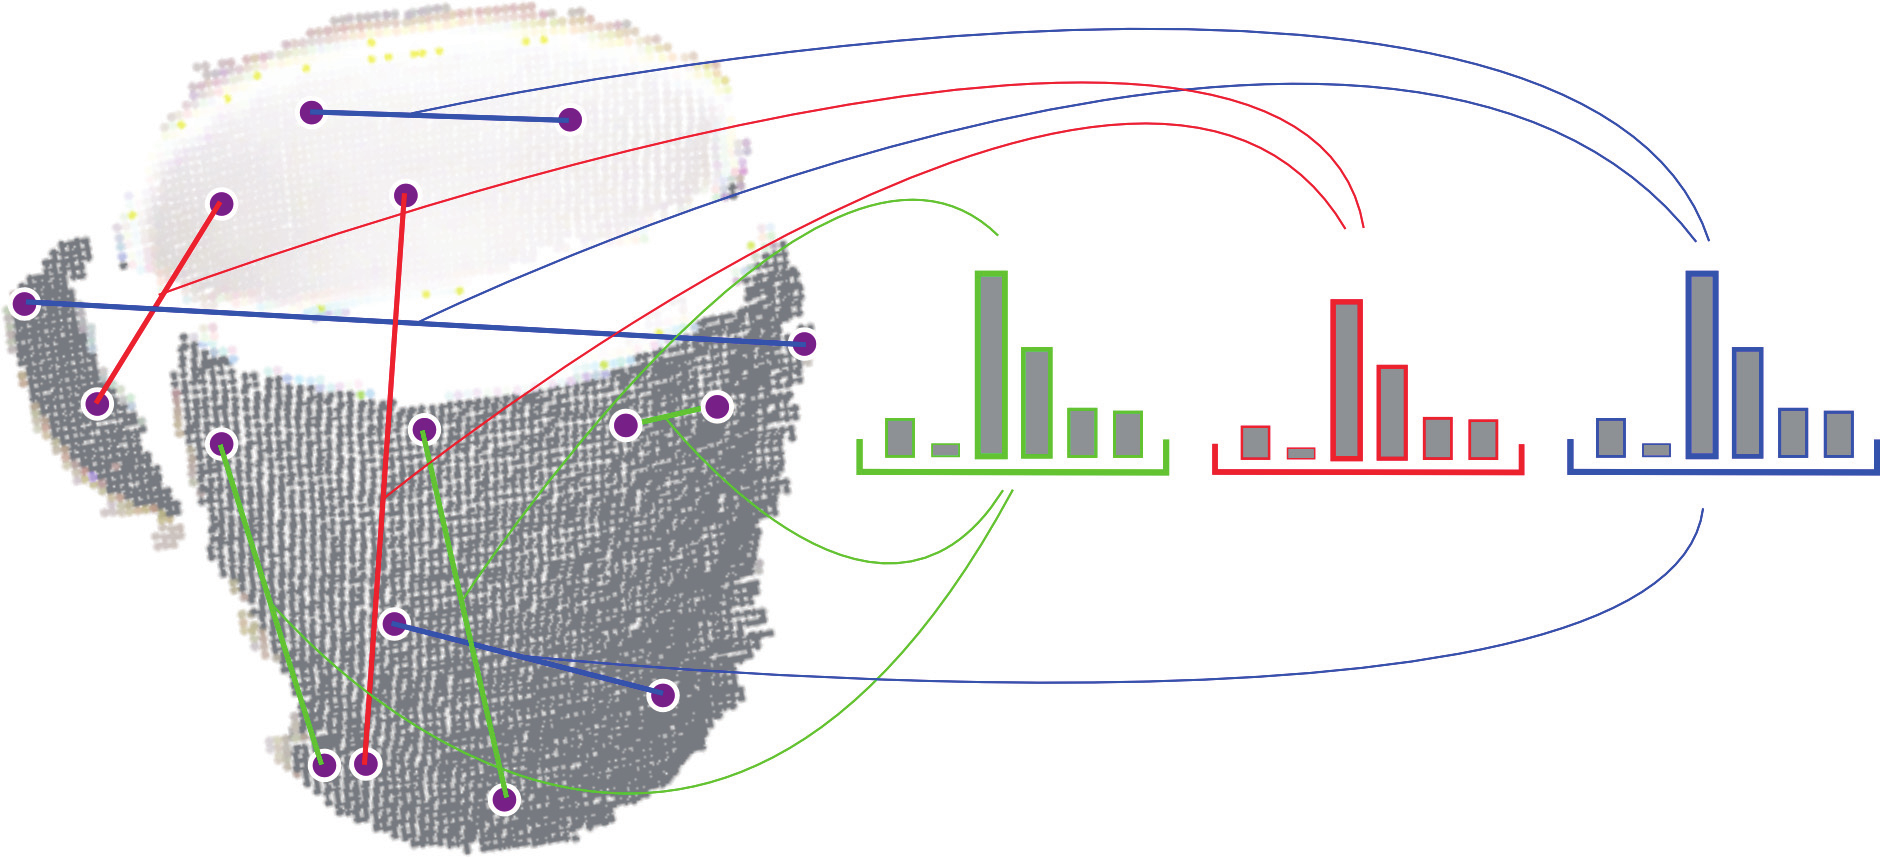
\includegraphics[width=0.23\textwidth]{images/wohl_onoff}
  }
  \subfloat[]{
    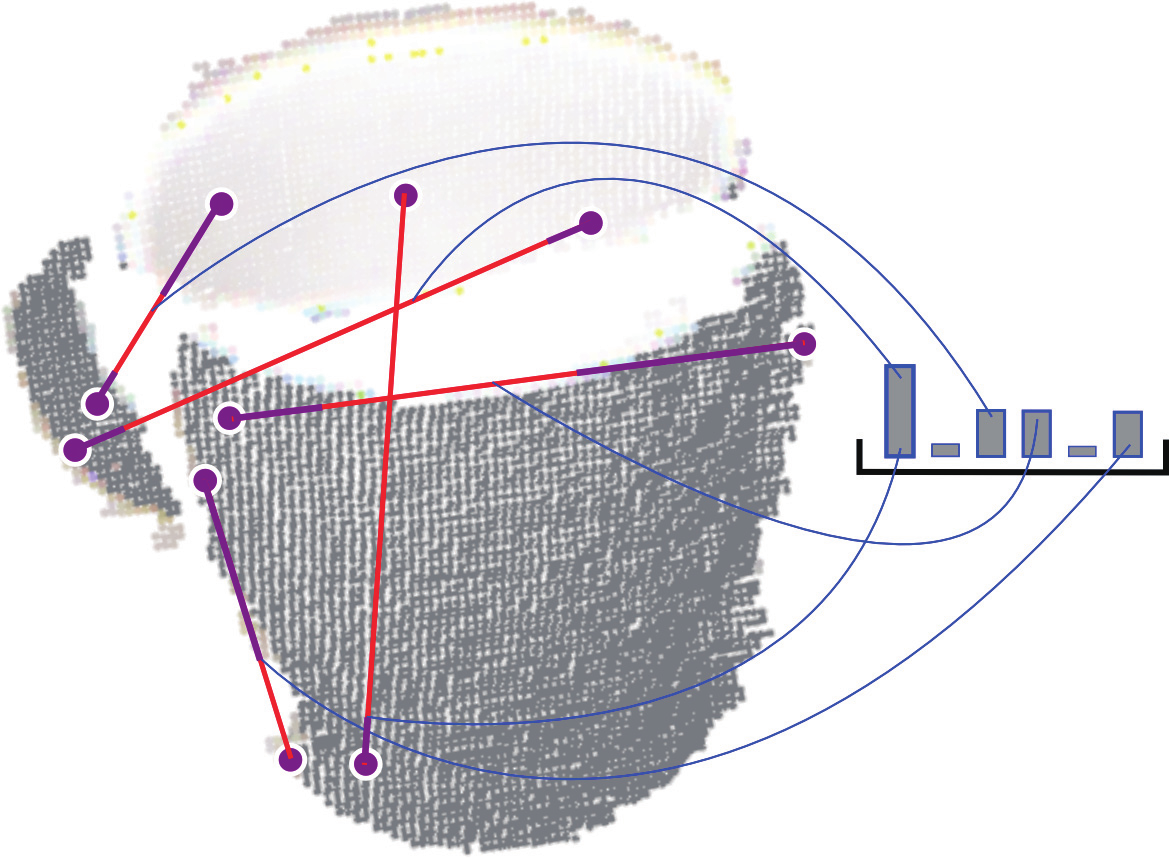
\includegraphics[width=0.23\textwidth]{images/wohl_ratio}
  }
  \subfloat[]{
    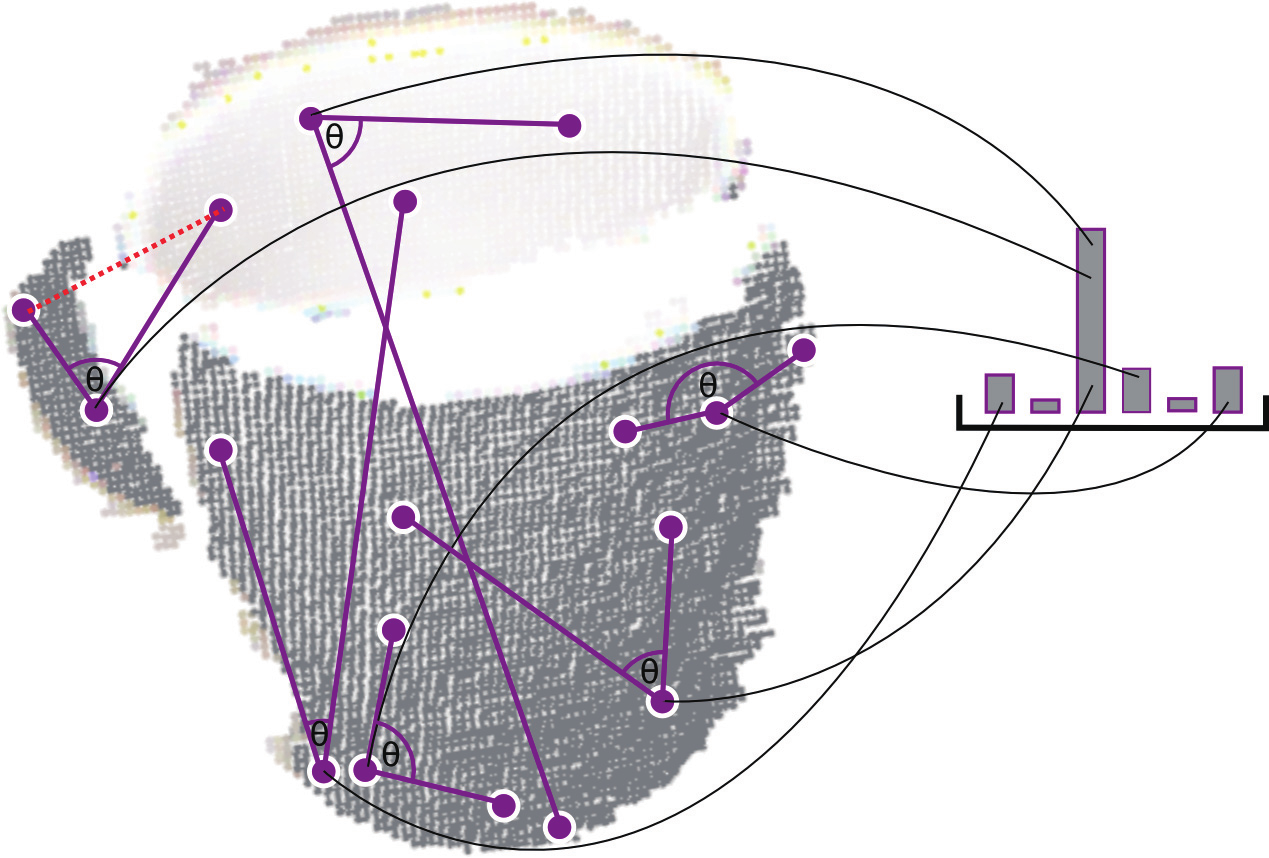
\includegraphics[width=0.23\textwidth]{images/wohl_a3}
  }
  \caption{Examples of the measures used to construct the Ensemble of Shape
    Functions histograms of \cite{wohlkinger2011ensemble}. a) Distance between
    points. b) Whether the points are on or off the model, or mixed. c) Ratio of
  line segments on and off the surface of the model. d) Angle between pairs of lines.}
  \label{fig:wohlESF}
\end{figure}
\section{Point Matching}
In \cite{chui2003new}, Chui and Rangarajan introduce an extension to ICP which
allows for non-rigid registration and improved robustness to outliers. In
contrast to ICP, their approach does not use the nearest-neighbour approach to
define correspondence. Instead, they use an alternating algorithm similar to
expectation maximisation. Annealing is used to prevent binary correspondences
when the algorithm is not yet close to the solution --- at the beginning there
is a large search range for correspondences, which gradually shrinks as the
temperature decreases.
\section{Model Matching}
\begin{figure}
  \centering
  \subfloat[Conformal factors. High value indicates high required deformation to
  sphere \cite{ben2008characterizing}.]{
    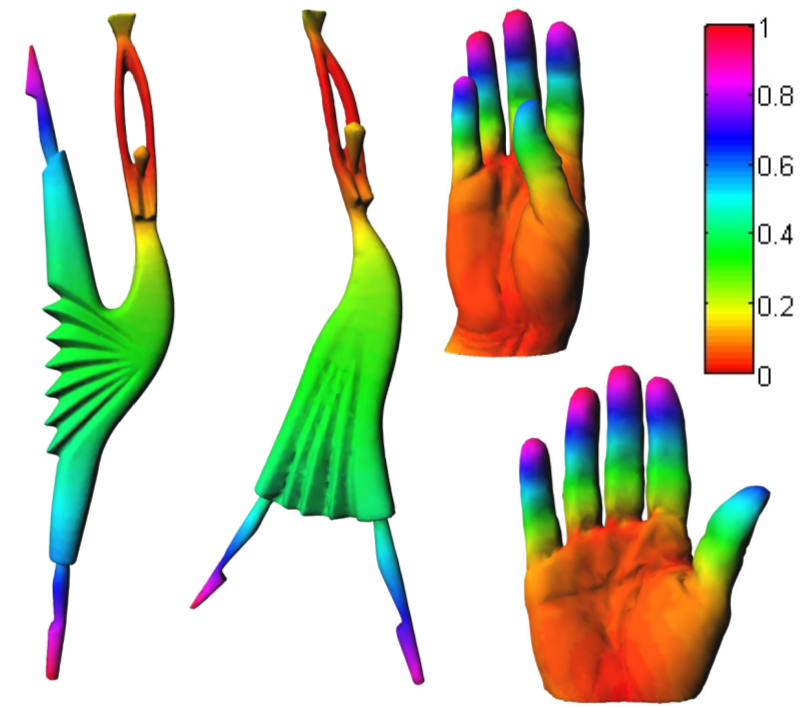
\includegraphics[width=0.48\textwidth]{images/conformal.png}
    \label{fig:conform}
  }
  \caption{Model matching approaches}
  \label{fig:modelmatch}
\end{figure}
In \cite{ben2008characterizing}, Chen et al. describe another approach to model
matching using conformal factors. This technique uses ideas from conformal
geometry, transforming the mesh of an object such that it has a uniform Gaussian
curvature. Information is stored about how much deformation is needed locally to
globally transform the object into a sphere --- this is the conformal factor.
The factor is based on a global computation on the whole mesh, as opposed to
per-vertex computations of the Gaussian curvature, which makes it much smoother
and appropriate for use in histograms. The histogram of a sample of the factors
is used as a descriptor, and is pose invariant, as seen in
Figure~\ref{fig:conform}. The authors say that it should be possible to use the
approach in partial model matching.
\section{Storing and Querying Descriptors}

\printbibliography
\end{document}